\documentclass[a4paper,oneside,article, titlepage]{article}
\usepackage[T1]{fontenc}
\usepackage{textcomp}
\usepackage[utf8]{inputenc}
\usepackage[danish]{babel}
\usepackage[garamond]{mathdesign}
\usepackage{tikz}
\usepackage{graphicx}

\DeclareTextFontCommand{\textfleur}
{\fontencoding{T1}\fontfamily{FleurCornerCaps}\selectfont}


\renewcommand{\ttdefault}{pcr} % bedre typewriter font
\renewcommand{\rmdefault}{ugm} % garamond


\usepackage{lettrine}

%\overfullrule=5pt

%\setsecnumdepth{part}

\title{Kravspecifikation til hjemmesideanalyse  \\
       \small{Førsteårsprojekt}}

\author
{
  Gruppe 1:\\
  Troels Henriksen (athas@sigkill.dk)\\
  Jesper Reenberg (reenberg@kampsax.dtu.dk)\\
  Martin Dybdal (dybber@dybber.dk)\\ \\
  Vejledere: Dina og Kasper
}


\setcounter{tocdepth}{3}
\setcounter{secnumdepth}{1}

\pagestyle{plain}

\date{\today}

\begin{document}
\maketitle
\tableofcontents
\newpage

\section{Baggrund}
\lettrine[lines=5,findent=0.5em,loversize=0.07,nindent=0em,image=true]%
{fairy}{aver man} en hjemmeside er det ofte fordi man gerne vil have
et budskab ud, hvad enten det er et firma eller en privatperson der
står bag. For at få sit budskab ud så effektivt som muligt bliver man
nødt til at gøre teksten man skriver så læsbar som muligt. Det er ikke
altid åbenlyst for en tekstforfatter hvor svær teksten vil være at
læse for en anden, især hvis forfatteren er vant til at skrive til en
anden målgruppe.  teksten på en del hjemmesider er derfor ikke så
tilgængelig som den kunne være.

Når man vil forfatte noget tekst er der en del der kan gå galt ---
eller i hvert fald mindske læsbarheden. Hvis man fx bruger
komplicerede ord, skriver langesætninger og laver stavefejl vil
læsbarheden falde drastisk. Man risikerer derved at budskabet man vil
sende når ud til færre mennesker.

Der er flere måder at forbedre læsbarheden af en tekst. Bl.a. har
typografi, farver og opsætning også indflydelse på hvor nem en tekst
er at læse.

\section{Til læseren}
\lettrine[lines=5,findent=0.5em,loversize=0.07,nindent=0em,image=true]%
{fairy}{æseren} af denne kravspecifikation bør være bekendt med rudimentær
HTML, XML og koncepterne bag tegnindkodning.
\\\\\\\\
Dokumentet består af følgende afsnit:
\begin{description}
\item \textbf{Formål og Målgruppe} --- forklaring af formålet med
  projektet er og hvilke forventninger vi vil stille til brugere af
  programmet.
\item \textbf{Analyse} --- beskrivelse af hvordan programmet kan
  laves, hvordan vi vil gøre og hvilke ting der skal tages specielt
  højde for.
\item \textbf{Prioritering} --- de prioriteter vores krav er inddelt
  i.
\item \textbf{Krav} --- gennemgang af de krav vi vil stille til
  programmet med angivet prioritet.
\item \textbf{Afhængigheder} --- her er de krav vist der afhænger af
  andre, hvis et krav skal implementeres så skal de krav det afhænger
  af være implementeret først.
\end{description}


\section{Formål}
\lettrine[lines=5,findent=0.5em,loversize=0.07,nindent=0em,image=true]%
{fairy}{æsbarheden } er noget af det vigtigste på en hjemmeside, og
for at hjælpe hjemmeside-forfattere vil vi konstruere et program der
kan analysere hjemmesider og hjælpe med at identificere passager hvor
læsbarheden ikke er i top. Programmet vil kun fokusere på selve
teksten, udseendet vil ikke blive vurderet. Hvis en hjemmeside bruger
ben dårlig skrifttype, så er det en designmæssig beslutning, som vi
ikke kan vurdere positivt eller negativt.

\section{Målgruppe}
En person i vores målgruppe er en hjemmesideskribent der er bekendt
med HTML. Personen har en professionel interessere i at teksten er
læsbar, således at vedkommende selv vil sætte sig ind i betydningen af
de udførte analysers resultater.

Programmet kan bruges på flere måder. En brugssituation er den
skitseret i afsnittet \textit{Baggrund} hvor en hjemmesideskribent vil
slå ned på noget tekst for at se om det er læsbart. En anden kunne
være en webmaster, som vil checke tekst skrevet af andre på tværs af
hele det website som han er ansvarlig for.

\section{Terminologi}
\lettrine[lines=5,findent=0.5em,loversize=0.07,nindent=0em,image=true]%
{saints}{g her} er så definitionen af nogle begreber vi bruger.
\\\\\\\\
\begin{description}
\item Websted --- en samling HTML-sider placeret på samme domæne. Et
  websted indeholder én eller flere \textit{sider}.
\item Side --- en enkelt HTML-side på et websted.
\item Sidesværhedsgrad --- et tal der angiver hvor svær en given side er
  at læse.
\end{description}

\section{Analyse}
\lettrine[lines=5,findent=0.5em,loversize=0.07,nindent=0em,image=true]%
{n}{år teksten} på en hjemmeside skal analyseres, så skal teksten på
siden først trækkes ud, da der er meget mere end blot tekst på en
hjemmeside. Vi definerer \textit{sidens tekst} som hjemmesidens
brødtekst, overskrifter og andet synligt tekst. Dog også tekst
der ikke er synligt, fx er der en speciel måde at definere det tekst
der skal vises når man har musen over et billede
(\texttt{title}). Tekst der bliver vist på denne måde er også en del
af \textit{sidens tekst}.

\subsection{Præsentation af resultater}
\lettrine[lines=5,findent=0.5em,loversize=0.07,nindent=0em,image=true]%
{n}{år man} skal analysere et større websted vil det ikke være muligt at
gå alle sidernes analyseresultater manuelt, og det er derfor relevant
for os at gøre det nemt at få et overblik over hvor der er plads til
forbedring. Vi vil derfor vise analyseresultatet som en liste over
alle de sider der findes på webstedet sammen med et resumé af deres
individuelle analyseresultater (lixtal, antal stavefejl, osv.).

For at gøre det endnu nemmere at finde sider der er særligt svære at
læse, vil vi lade listen af undersider være sorteret efter deres
sværhedsgrad. Dette betyder at vi skal have en specifik værdi for
sværhedsgrad, som vi kan sortere efter. Denne værdi kalder vi
\textit{sidesværhedsgrad} og den skal beregnes ved at kombinere
resultater fra flere af de analysemetoder vi vil understøtte (se krav
2.1--2.5). Algoritmen der kombinerer resultaterne skal sørge for
at resultaterne bliver ligebyrdige, da resultaterne fra de forskellige
analyser er på vidt forskellige skalaer (se krav 2.5).

En enkelt side kan have meget tekst, hvis man ikke får at vide hvor på
siden problemet er størst, så er programmet ikke til megen hjælp. Fra
oversigtssiden skal man derfor kunne klikke sig ind på
analyseresultatet for en specifik side, som indeholder mere detaljeret
information, bl.a. en liste over al tekst på siden, der er sat med
farver som angiver de enkelte sætningers sværhedsgrad. For flere
detaljer, se krav 2.

\subsection{Valg af interface}
Det åbenlyse valg af interface ville være en webapplikation ---
alligevel har vi valgt at implementere programmet som et
kommandolinjeprogram som genererer HTML-filer. Dette valg blev truffet
for at vi kunne bruge mere tid på at udvikle en god måde at analysere
hjemmesider på, og ikke skulle bruge tid på at lave et avanceret
interface. Ydermere vil det sandsynligvis tage betragtelig tid at
analysere blot middelstore hjemmesider --- en webapplikation ville måske
time ud før den blev færdig, og brugeren ville helt sikkert hurtigt
blive træt af at vente. Med et kommandolinjeprogram vil programmet
være sværere at bruge for en del personer, men dog ikke sværere end
alle andre kommandolinjerprogrammer, og altså overkommeligt for
rimeligt tekniske brugere, især de, der benytter sig af Unix-systemer
til dagligt. Da vores outputformat er HTML er det ydermere relativt
let at lave et webinterface til programmet senere. For at omgå
tidligere nævnte køretidsproblemer, kunne dette interface være
opbygget omkring ``bestillinger'' af analyser, hvor webinterfacet
bruger kommandolinjeprogrammet til at analysere den ønskede
hjemmeside, og beder brugeren om at komme tilbage senere (hvis
analysen forventes at tage meget lang tid kunne der endda sendes en
email når resultatet er klart). At præsentere brugeren for resultatet
kunne trivielt gøres ved at kopiere program-output-filerne til en
serverplacering som er tilgængelig via brugerens browser.

\subsection{Håndtering af HTML}
På Internettet støder man på imponerende mange forskellige HTML-sider,
at håndtere dem alle er noget som selv de størst og ældste webbrowsere
kan have svært ved. Ældre HTML-sider benytter gamle standarder, de
færreste sider overholder alle standarderne, visse sider er skrevet
halvvejs i Javascript, gør brug af indlejrede objekter (som
f.eks. Java eller Flash), visse XHTML-sider gør brug af avancerede
XML-features, osv. Det ville være håbløst for os at forsøge at skrive
et program til at håndtere alt dette i den afsatte tid, og vi vælger
derfor at begrænse os til simpel HTML og XHTML der er nogenlunde
korrekt. Vi håndterer ikke indlejrede objekter, Javascript,
stylesheets eller avancerede XML-features som transformationer, DTD'er
og namespaces. Ydermere kan sider indkodes i en af mange forskellige
tegnkodninger, noget som vi ikke har store chancer for at understøtte
korrekt. Vi vælger derfor at begrænse vores understøttelse af
tekstindkodnings-standarder (se krav 8.1).

\subsection{Semantisk information i HTML}
HTML som format er specielt, fordi det ud over at indeholde
information om hvordan teksten skal se ud (typografisk data), også
indeholder data om tekstens betydning (semantik). Selvom mange sider
undlader at bruge HTML's brede udvalg af semantisk betydningsfulde
tags mener vi alligevel at det er en fordel at drage nytte af dem, når
det er muligt. Chancen for at behandling af de semantisk betydende
tags medfører en ukorrekt analyse, pga. ukorrekt brug af tags'ne på
siden, er lille, idet HTML-sider i højere grad er præget af mangel på
semantisk betydningsfulde tags, end direkte misbrug af dem. At udnytte
forekomsten i disse tags i vores analyse, og derved være i stand til
at give en mere præcis og brugbar analyse for sider der korrekt bruger
HTML's semantisk betydende tags, fungerer også som opfordring til at
hjemmesideforfattere begynder at bruge disse tags - udover at hjælpe
vores program, letter det også livet for f.eks. blinde besøgende som
benytter sig af netlæsere.

\section{Prioritering}
\lettrine[lines=5,findent=0.5em,loversize=0.07,nindent=0em,image=true]%
{saints}{pdelt} i tre prioritets-kategorier har vi kravene gjort.
\\\\\\\\
\begin{description}
\item Uundværlige --- krav der skal opfyldes af en
  prototype. Krav med denne prioritet dækker uundværlig
  funktionalitet, hvis tab ville resultere i at programmet var nærmest
  ikke-funktionelt.
\item Vigtige --- krav der beskriver funktionalitet som vil
  gøre programmet usædvanligt og interessant for brugerne. Krav med
  denne prioritet forventes at være opfyldt i den endelige
  implementation.
\item Mindre vigtige --- krav der ikke er nødvendige for at
  programmet kan bruges, men som kunne være rare at have med i en
  senere revision. Implementationen skal altså tage højde for at disse
  krav skal kunne implementeres senere hen.
\end{description}

\newpage

\section{Krav til funktionalitet}
\subsection{Krav 1: Analyse af et helt websted}
Man skal kunne foretage en overordnet analyse af et helt
websted. Dvs. alle undersider (som kan nås via links fra forsiden)
skal medtages og der skal produceres information om dem (se Krav 2.1).

\begin{description}
\item \textbf{Eksempel:}
  Hvis man eksempelvis beder om en analyse af hele diku.dk, så skal
programmet finde frem til alle undersider (diku.dk/diku/,
diku.dk/forskning/ osv.) og udføre en komplet tekstanalyse af hver af
disse undersider, samt producere en oversigt over alle undersiderne.

\item \textbf{Baggrund:} \textit{Krav fra opgavestiller.} For en webmaster er
  det yderst relevant at udføre tekstanalyse på et helt websted, for
  derefter at gribe ind på de undersider hvor det er nødvendigt. På
  selv et middelstørrelses-websted kan det være uoverskueligt at
  analysere hver enkelt underside manuelt.

\item \textbf{Prioritet:} Uundværlig.
\end{description}

\subsubsection {Krav 1.1: Respekter robots.txt}
Programmet skal respekterer eventuelle robots.txt
\footnote{http://www.robotstxt.org/wc/robots.html} filer. Det skal
være muligt at slå dette fra.

\begin{description}
\item \textbf{Eksempel:} Hvis man beder om en analyse af
  http://da.wikipedia.org så skal programmet hente filen
  http://da.wikipedia.org/robots.txt og programmet skal så lade være
  med at analysere de hjemmesider som den ikke må analysere.

\item \textbf{Baggrund:} \textit{Krav fra opgavestiller.} Vi vil
  nødigt chikanere nogle ved at lade vores program crawle på sider
  hvor det er uønsket. Vi vil dog heller ikke forhindre vores program
  i at virke, bare fordi man ikke ønsker at blive indekseret af
  søgemaskiner.
\item \textbf{Prioritet:} Uundværlig.
\end{description}

\subsubsection{Krav 1.2: Dybde af crawling}
Det skal være muligt at angive den dybde af hyperlinks fra hovedsiden
som analyseprogrammet skal følge, hvis man sætter det til at analysere
en hel side. At sætte dybden til 0 har den effekt at kun den side man
direkte angiver til programmet (oftest websitets forside) vil blive
analyseres.

\begin{description}
\item \textbf{Eksempel:} Man kan f.eks. sætter en analyse i gang med
  en maksimal dybde på 5 links. Så skal sider der er længere end 5
  links væk ikke analyseres.

\item \textbf{Baggrund:} \textit{Krav stillet af gruppen.} Dette har
  den fordel at hvis man sætter den til at analysere wikipedia.org så
  vil programmet ikke dø. Wikipedia.org er så stort et websted at
  programmet vil kunne komme til at opbruge al hukommelsen.
\item \textbf{Prioritet:} Vigtig.
\end{description}

\subsection{Krav 2: Analysemetoder}
Vi vil understøtte de følgende analysemetoder til at analysere teksten
på en side.

\begin{description}
\item \textbf{Eksempel:} Når f.eks. undersiden diku.dk/forskning/ skal
  analyseres skal programmet foretage de nedenstående tekstanalyser på
  sidens tekst.

\item \textbf{Baggrund:} \textit{Krav fra opgavestiller.} Den
  overordnede analyse omtalt i krav 1 hjælper med at finde de sider
  der har brug for at blive rettet, dette sker ved at præsentere et
  resumé af resultaterne fra de nedenfor benævnte analysemetoder.
\item \textbf{Prioritet:} Uundværlig.
\end{description}

\subsubsection{Krav 2.1: Læsbarhedsindeks, LIX}
Programmet skal kunne udregne lixtal.

\begin{description}
\item \textbf{Eksempel:} Givet en tekst skal programmet kunne beregne
  LIX-tallet for teksten.
\item \textbf{Baggrund:} \textit{Krav stillet af gruppen.} LIX er en
  populær og kendt algoritme til at afgøre sværhedsgraden af en given
  tekst. Det er derfor relevant at bruge denne til at afgøre
  læsesværhedsgraden af teksten på sider.
\item \textbf{Prioritet:} Uundværlig.
\end{description}


\subsubsection{Krav 2.2: Flesch-Kincaid Readability Test (FKRT)}
Programmet skal kunne udføre Flesch-Kincaid Readability Test.

\begin{description}
\item \textbf{Eksempel:} Givet en tekst skal programmet kunne beregne
  FKRT for teksten.
\item \textbf{Baggrund:} \textit{Krav stillet af gruppen.} FKRT er en
  tekstanalysealgoritme som især vægter sætningslængde. Se nedenfor
  for uddybende begrundelse.
\item \textbf{Prioritet:} Vigtig.
\end{description}

\subsubsection{Uddybet begrundelse for krav 2.1 og 2.2}
De to analysemetoder supplerer hinanden godt, idet LIX primært er
baseret på ordlængde, hvorimod FKRT også tager sig af
sætningslængde. Sammen giver de et rimeligt billede af tekstens
sværhedsgrad. Det er endnu ikke besluttet om resultatet for de to
analysemetoder skal kombineres eller vises separat fra hinanden.

\subsubsection{Krav 2.3: Stavekontrol}
Programmet skal kunne finde stavefejl. Som udgangspunkt skal
programmet kun kunne finde stavefejl i danske tekster (se krav
2.1.3.1).

Stavekontrollen vil ikke indgå i beregningen af sidesværhedsgraden, men
kun blive brugt til at vise stavefejl da dette vil være alt for svært
at håndtere (fx hvis en dansk side indeholder mange engelske termer).
\begin{description}
\item \textbf{Eksempel:} Givet en tekst skal programmet kunne tjekke
  for stavefejl i forhold til det danske sprog.
\item \textbf{Baggrund:} \textit{Krav stillet af gruppen.} 
\item \textbf{Prioritet:} Vigtig.
\end{description}

\subsubsection{Krav 2.3.1: Flere sprog}
Programmet skal kunne udvides til et arbitrært antal sprog (defineret
ved deres sprogkode).
\begin{description}
\item \textbf{Eksempel:} Ved en analyse kan programmet lade brugeren
  vælge hvilket sprog siden er på eller selv prøve at finde ud af
  hvilket sprog der er tale om (ved at se på specielle HTML-tags).
\item \textbf{Baggrund:} \textit{Krav stillet af gruppen.}
\item \textbf{Prioritet:} Mindre vigtig.
\end{description}

\subsubsection{Krav 2.4: Gentagne ord}
Programmet skal kunne finde gentagne ord.
Denne analyse skal heller ikke påvirke sidesværhedsgraden.

\begin{description}
\item \textbf{Eksempel:} Givet en tekst skal programmet kunne finde
  gentagelser af samme ord.
\item \textbf{Baggrund:} \textit{Krav stillet af gruppen.} Det er
  yderst sjældent at det er med vilje at en tekst indeholder to på
  hinanden følgende identiske ord, men det er tværtimod en fejl man
  ofte kommer til at lave, især hvis man bliver distraheret under
  skrivningen.
\item \textbf{Prioritet:} Mindre vigtig.
\end{description}

\subsubsection{Krav 2.5: Beregning af sidesværhedsgrad}

For hver enkelt side beregnes der et entydigt tal, der angiver sidens
tekstmæssige sværhedsgrad. Dette tal betegnes sidens
\textit{sidesværhedsgrad}. LIX og FKRT-analyser resulterer i en talværdi
der angiver tekstens sværhedsgrad. Da disse talværdier ikke befinder
sig på samme skala, er det nødvendigt at finde en vægtningsfaktor som
kan sikrer at en af de to algoritmer ikke vil have en uforholdsmæssigt
stor indflydelse på sidesværhedsgraden. Denne vægtningsfaktor er endnu
ikke kendt, men vil bestemmes ved at udføre LIX og FKRT-analyser på en
mængde repræsentative tekster og sammenligne talresultaterne

\begin{description}
\item \textbf{Eksempel:} Programmet kan eksempelvis vægte FKRT med
  80\% i forhold til LIX i sidesværhedsgraden. 
\item \textbf{Baggrund:} \textit{Krav stillet af gruppen.} Når man
  gennemgår et websted for at finde undersider med en uacceptabelt høj
  tekst\-sværhedsgrad er det praktisk at tekst\-sværhedsgraden på hver
  enkelt underside kan angives med en enkelt talværdi - f.eks. for at
  gøre det muligt at sortere siderne. Sidesværhedsgraden fungerer som
  denne talværdi.
\item \textbf{Prioritet:} Vigtig.
\end{description}

\subsection{Krav 3: Analyse baseret på HTML-tags.}
Den semantiske information som HTML-tags angiver skal bruges til at
påvirke de andre analyser.

\begin{description}
\item \textbf{Eksempel:} Se underkravene for eksempler.
\item \textbf{Baggrund:} \textit{Kravene er stillet af gruppen.} HTML
  som format er specielt, fordi det udover at indeholde typografisk
  information om teksten, også indeholder semantisk information. At
  udnytte denne semantiske information kan derfor resultere i et mere
  præcist og brugbart resultat, end en simpel tekstanalyse, som blot
  smider informationen væk. \textit{Krav stillet af gruppen}.
\item \textbf{Prioritet:} Mindre vigtig.
\end{description}

\subsubsection{Krav 3.1: \texttt{em} og \texttt{strong}}

\texttt{em} og \texttt{strong} indikerer særligt vigtig tekst, og
sætninger indeholdende disse er således vigtigere end andre for
tekstens samlede læsbarhed, og skal vægtes højere i beregningen af
sidesværhedsgraden.

\begin{description}
\item \textbf{Eksempel:} Sætninger indeholdende \texttt{em} eller
  \texttt{strong}-tags skal bidrage mere end andre sætninger i
  beregningen af en sides sidesværhedsgrad.
\item \textbf{Prioritering:} Mindre vigtig.
\end{description}

\subsubsection{Krav 3.2: \texttt{hN}}

Overskrifter, som markeres med \texttt{hN}-familien af tags, udgør
relativt lidt af en sides tekst, men har en langt højere synlighed end
en vilkårlig almindelig sætning, og bør derfor vægtes højere i
beregningen af sidesværhedsgraden.

\begin{description}
\item \textbf{Eksempel:} Sætninger i overskrifter skal vægtes højere
  end andre sætninger i beregningen af en sides sidesværhedsgrad.
\item \textbf{Prioritering:} Mindre vigtig.
\end{description}

\subsubsection{Krav 3.3: \texttt{abbr} og \texttt{acronym}}
\texttt{abbr} og \texttt{acronym}-tags bruges til at markere at et
givent ord er en forkortelse. Da forkortelser ofte ikke kan
stavekontrolleres (især forkortelser for virksomhedsnavne og tekniske
termer) er det en fordel ikke at markere evt. ukendte forkortelser som
stavefejl.

\begin{description}
\item \textbf{Eksempel:} Når programmet støder på et ord, som via HTML
  er angivet som værende en forkortelse, vil ordet ikke blive
  stavekontrolleret.
\item \textbf{Prioritering:} Mindre vigtig.
\end{description}

\subsubsection{Krav 3.4: Citater skal ikke analyseres.}
Tekst i \texttt{q} eller \texttt{blockquote}-tags
  (dvs. citationer) skal ikke analyseres, men dog stavekontrolleres,
  da det ikke formodes at disse kan skrives om.

\begin{description}
\item \textbf{Eksempel:} Hvis der optræder et citat i den tekst der
  skal analyseres, så skal teksten ikke tages med i lixberegningen,
  FKRT mv. kun stavekontrol skal udføres.
\item \textbf{Prioritering:} Mindre vigtig.
\end{description}

\subsubsection{Krav 3.5: Tekst i andre sprog angivet med
  (\texttt{lang})}
Tekst, angivet som et sprog (via \texttt{lang}-tagget) som ikke er
understøttet, skal ikke stavekontrolleres.

\begin{description}
\item \textbf{Eksempel:} Hvis der indgår et citat på latin i teksten,
  så skal citatet kontrolleres for stavefejl med en latinsk
  stavekontrol. Hvis der ikke er nogen stavekontrol er til latin, så
  skal citatet slet ikke stavekontrolleres.
\item \textbf{Prioritering:} Mindre vigtig.
\end{description}

\subsubsection{Krav 3.6: \texttt{kbd}, \texttt{var} og \texttt{code}}
Visse tags, som f.eks. \texttt{kbd}, \texttt{var}, og \texttt{code}
angiver at teksten ikke indeholder almindelig tekst, og derfor ikke
skal analyseres.

\begin{description}
\item \textbf{Eksempel:} Er der f.eks. angivet at et afsnit er kode
  med \texttt{code}-tagget, så skal det ikke analyseres.
\item \textbf{Prioritering:} Mindre vigtig.
\end{description}

\subsubsection{Krav 3.7: \texttt{bdo}}
\texttt{bdo}-tagget kan bruges til at angive, at teksten skal skrives
fra højre mod venstre (eller omvendt). I dette tilfælde skal
bogstaverne i teksten vendes om før der udføres stavekontrol.

\begin{description}
\item \textbf{Eksempel:} Arabisk tekst skrives fra højre til venstre,
  hvis det skal analyseres, så skal teksten først vendes den
  anden vej.
\item \textbf{Prioritering:} Mindre vigtig.
\end{description}

% Der tages forbehold for senere tilføjelse af andre tags der skal
% specialbehandles.

\subsection{Krav 4: Konfiguration af analyse}
Programmet skal gøre det muligt at angive hvor omfattende en analyse
der skal foretages og lade brugeren indstille de enkelte
analysemetoder. Man skal kunne indstille:

\begin{itemize}
\item Hvilke analyser der skal udføres.
\item Hvilke dele af siden der skal medtages, baseret på
  HTML-elemen\-ter\-nes \texttt{id} og \texttt{class}-attributter. Så man
  fx kan udelukke brugerkommentarer fra analysen.
\end{itemize}

\begin{description}
\item \textbf{Eksempel:} Det kan fx være muligt at angive hvilke tjek
  der skal foretages (fx stavekontrol eller lix-beregning) og hvilke
  dele af siden der skal medtages i analysen. Fx skal citater og
  tabel-data måske udelades. Man kan også forestille sig at man vil
  ændre på hvordan overskrifter skal vægtes i analysen.
\item \textbf{Baggrund:} \textit{Krav stillet af gruppen.}
\item \textbf{Prioritet:} Mindre Vigtig.
\end{description}

\section{Krav til interface}

\subsection{Krav 5: Kommandobaseret interface}
Programmet vil være udformet som et kommandolinjeværktøj, og
interfacet vil bestå af kommandolinjeparametre. Programmet vil som
minimum tage en URL som parameter, og vil derudover understøtte
parametre til at kontrollere programmets specifikke opførsel -
f.eks. de i krav 1 og 2 nævnte to forskellige
analysefremgangsmåder.
\begin{description}
\item \textbf{Eksempel:} Hvis programmet hedder ``textanalyse'' så
  kunne programmet fx laves så det kan sættes til analysere diku.dk
  med:

  \texttt{./textanalyse http://diku.dk/}

\item \textbf{Baggrund:} \textit{Krav stillet af gruppen.} At
  implementere interfacet som et kommandolinjeprogram sikrer at vi har
  mere tid til at implementere effektive analysemetoder, og at det vil
  være overkommeligt at lave et grafisk interface baseret på
  kommandolinjeværktøjet senere hen.
\item \textbf{Prioritet:} Uundværlig.
\end{description}

\subsection{Krav 6: Resultater i HTML-format.}
Programmet skal generere HTML-filer der viser resultatet af en
analyse. Der genereres en index-fil der fungerer som indgang til
resten af analysen. Dette index indeholder en liste over alle de
undersider der er blevet analyseret, samt et resumé af deres
analyseresultat (f.eks. deres sidesværhedsgrad - evt. er listen over
undersider sorteret efter denne sidesværhedsgrad). Der bliver også
genereret en HTML-fil for hver analyseret underside - denne fil
indeholder en detaljeret analyse, bl.a. bestående af al tekst på
siden, hvor hver sætning er sat med farver alt efter hvor svær den er
at læse. På disse sider fremgår de konkrete LIX og FKRT-resultater
også, i stedet for blot at vise sidesværhedsgraden. Samtidigt fremgår
resultatet af stavekontrollen også. Fra index-sidens liste over
undersider går der links til disse HTML-resultat-filer.

\begin{description}
\item \textbf{Eksempel:} Programmet kan fx lave en fil ved navn
  ``index.html'', der indeholder en liste over alle undersiderne
  sorteret efter sidesværhedsgrad. Når man klikker på en underside i
  listen kommer man ind på en anden (af programmet genereret)
  HTML-side der indeholder yderligere oplysninger om den underside man
  klikkede på. Fx kan der vises stavefejl og afsnit med høje lixtal.

\item \textbf{Baggrund:} \textit{Krav stillet af gruppen.}  Dette er
  for at kunne lave mere avanceret visualisering af
  analyseresultatet. At generere HTML-filer kan også lette
  implementationen af et eventuelt senere web\-appli\-kations-baseret
  interface.
\item \textbf{Prioritet:} Vigtig.
\end{description}


\section{Krav til implementationen}

\subsection{Krav 7: Platform}
Programmet skal kunne køre på GNU-baserede Linux maskiner. Dette er
for at minimere antallet af systemkonfigurationer som skal testes.

\begin{description}
\item \textbf{Eksempel:} Programmet skal fx kunne køre på DIKUs maskiner.

\item \textbf{Baggrund:} \textit{Krav stillet af gruppen.} 
\item \textbf{Prioritet:} Vigtig.
\end{description}

\subsection{Krav 8: Håndtering af HTML/XHTML}
Programmet skal håndtere sider der overholder de gældende HTML
og XHTML standarder. Dog vil vi begrænse mængden af XHTML der skal
understøttes. Vi vil kun implementere den delmængde af XML der er
løftet næsten direkte fra SGML, hvilket er tilstrækkeligt til langt
den største part af XHTML-dokumenter.

Dette betyder også at der skal tages speciel hånd om nogle tags der
kan have indhold der kan ødelægge parsingen (eksempelvis
\texttt{<style>}, \texttt{<script>} og HTML-kommentarer).

\begin{description}
\item \textbf{Eksempel:} Dette krav betyder at en side der ikke
  overholder standarderne ikke altid vil blive analyseret korrekt, dog
  kan programmet evt. prøve at gætte på hvad der menes hvis der
  mangler et afsluttende tags og lignende.

\item \textbf{Baggrund:} \textit{Krav stillet af gruppen.} Vi vil ikke
  stille krav om at vi kan analysere lige netop den tekst der vises i
  browsere, for alle browsere har en meget stor fejlhåndtering der
  prøver at gætte på hvad man mener når man skriver forkert formateret
  HTML. Dette vil kræve for meget tid. Vi begrænser altså til
  dokumenter der er formateret korrekt.
\item \textbf{Prioritet:} Uundværlig.
\end{description}


\subsubsection{Krav 8.1: Indkodning}
Kun sider indkodet i ASCII eller Moscow ML's indbyggede indkodning
(sandsynligvis ISO-8859-1/Latin-1 på de fleste maskiner)
understøttes. Det kunne være rart også at understøtte UTF-8, og bruge
den indkodning som HTML-siden ønsker, men af simplicitetshensyn er
dette ikke et konkret krav.

\begin{description}
\item \textbf{Eksempel:} Hvis programmet bliver bedt om at analysere
  hjemmesider i UTF-8 format, så er det ikke et krav at programmet
  opfører sig korrekt.

\item \textbf{Baggrund:} \textit{Krav stillet af gruppen.} Dette krav
  er for at holde fokus, da implementationen af indkodnings-håndtering
  hurtigt kan lægge beslag på en tidsmængde som er ude af proportioner
  med hvad en sådan indkodnings-understøttelse ville give af fordele.
\item \textbf{Prioritet:} Vigtig.
\end{description}

\section{Illustration af afhængigheder}
\textit{For overskuelighedens skyld er krav uden afhængigheder
  udeladt.}

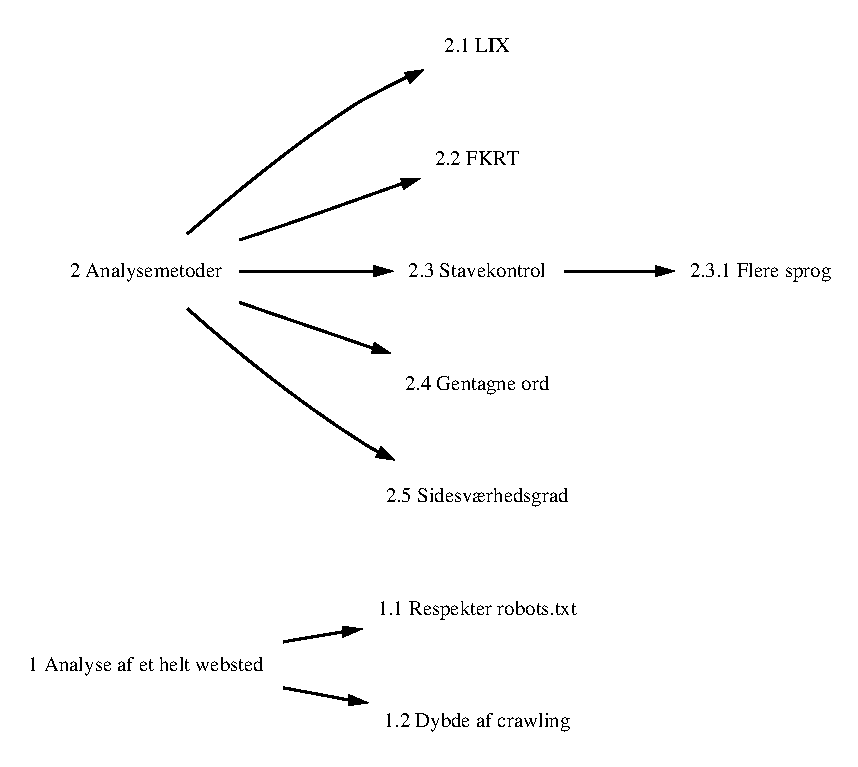
\includegraphics{kravill1.pdf}
\newpage
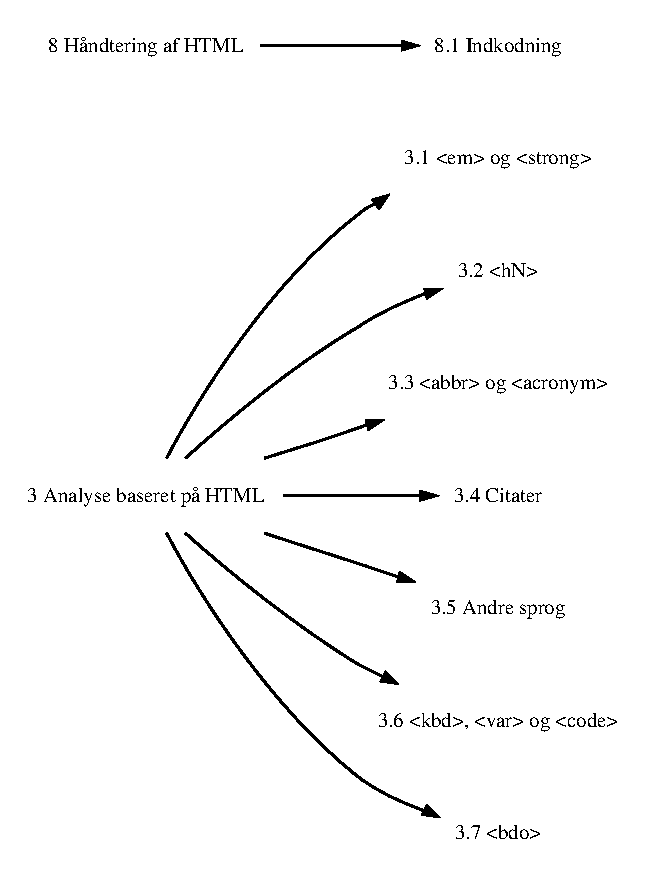
\includegraphics{kravill2.pdf}


% \begin{tikzpicture}
%   [parent anchor=east,child anchor=west,grow=east]
%     \tikzstyle{level 1}=[level distance=50mm]

%     \node {1 Analyse af et helt websted}
%         child { node {1.1 Respekter robots.txt} }
%         child { node {1.2 Dybde af crawling} }
%     ;
% \end{tikzpicture}

% \vspace{0.3cm}

% \begin{tikzpicture}
%   [parent anchor=east,child anchor=west,grow=east]
%     \tikzstyle{level 1}=[level distance=40mm]
%     \tikzstyle{level 2}=[level distance=35mm]

%     \node {2 Analyse af en konkret side}
%         child
%         { 
%           node {2.1 Analysemetoder}
%           child { node {2.1.1 LIX} }
%           child { node {2.1.2 FKRT} }
%           child { node {2.1.3 Stavekontrol}
%                   child { node {2.1.3.1 Flere sprog} }
%           }
%           child { node {2.1.4 Gentagne ord} }
%           child { node {2.1.5 Sidesværhedsgrad}}
%         }
%         child
%         { 
%           node {2.2 Analyse baseret på HTML}
%           child { node {2.2.1 \texttt{em} og \texttt{strong}} }
%           child { node {2.2.2 \texttt{hN} } }
%           child { node {2.2.3 \texttt{abbr} og \texttt{acronym}} }
%           child { node {2.2.4 Citater }}
%           child { node {2.2.5 Andre sprog (\texttt{lang})} }
%           child { node {2.2.6 \texttt{kbd}, \texttt{var} og \texttt{code}} }
%           child { node {2.2.7 \texttt{bdo}}}
%         }
%     ;
% \end{tikzpicture}

\end{document}
